%% LyX 2.0.6 created this file.  For more info, see http://www.lyx.org/.
%% Do not edit unless you really know what you are doing.
\documentclass[twocolumn,english]{paper}
\usepackage[T1]{fontenc}
\usepackage[latin9]{inputenc}
\usepackage[letterpaper]{geometry}
\geometry{verbose,tmargin=2.65cm,bmargin=2.65cm,lmargin=2.65cm,rmargin=2.65cm}
\setlength{\parindent}{0bp}
\usepackage{amsthm}
\usepackage{amsmath}
\usepackage{graphicx}
\usepackage{setspace}
\onehalfspacing

\makeatletter

%%%%%%%%%%%%%%%%%%%%%%%%%%%%%% LyX specific LaTeX commands.
%% A simple dot to overcome graphicx limitations
\newcommand{\lyxdot}{.}


%%%%%%%%%%%%%%%%%%%%%%%%%%%%%% Textclass specific LaTeX commands.
\numberwithin{equation}{section}
\numberwithin{figure}{section}

\makeatother

\usepackage{babel}
\begin{document}

\title{This is Article}


\author{Christian Poveda Ruiz}
\maketitle
\begin{abstract}
FIXME: Write abstract
\end{abstract}

\section{Introduction}

FIXME: Multidark

FIXME: NFW profile

FIXME: MCMC


\section{State of Art}


\section{What did I do?}

FIXME: Which simulation? $m=1.7\times10^{11}\ M_{\odot}$ 

$ $

In order to obtain a mass profile for each halo in funcion of the
radius, the center of each halo must be calculated. However the center
of mass will not give an accurate position for the center because
some haloes are highly irregular, is more convenient to take the gravitational
potential for each particle

\[
\phi\left(\boldsymbol{r}_{n}\right)=-\sum_{j\neq i}\frac{1}{\left\Vert \boldsymbol{r}_{n}-\boldsymbol{r}_{j}\right\Vert }
\]
Take $\boldsymbol{r}_{0}=\min\left(\phi\left(\boldsymbol{r}_{n}\right)\right)$
as the center then define new coordinates $\boldsymbol{r}_{n}^{\prime}=\boldsymbol{r}_{0}-\boldsymbol{r}_{n}$,
this $\boldsymbol{r}_{0}$ will be in the most relevant region for
the dynamics of each halo. Organizing the $\left\{ \boldsymbol{r}_{n}^{\prime}\right\} $
in crescent order, the accumulated mass for each $\boldsymbol{r}_{n}^{\prime}$
will be $m_{n}=nm$.

$ $

FIXME: Mass profile of a halo

$ $

The last part of the process consists in fitting the NFW mass profile
to the $m_{n}$ data using the Metropolis-Hastings algorithm to sample
the Likelihood ${\cal L}\left(\rho_{0},r_{s}\right)=\exp\left(-\frac{1}{2}\chi^{2}\left(\rho_{0},r_{s}\right)\right)$,
where $\chi^{2}\left(\rho_{0},r_{s}\right)=\sum\limits _{n}\left|m_{n}-m\left(\boldsymbol{r}_{n}^{\prime},\rho_{0},r_{s}\right)\right|^{2}$,
and take the values of $\rho_{0}$ and $r_{s}$ where the Likelihood
is maximum.


\section{Results}


\subsection{Trial Problem with several Generated Halos }

FIXME: I tested it with HaloGenerator


\subsection{Results from the simulation}

FIXME: Plot with error bars

\begin{figure}
\begin{centering}
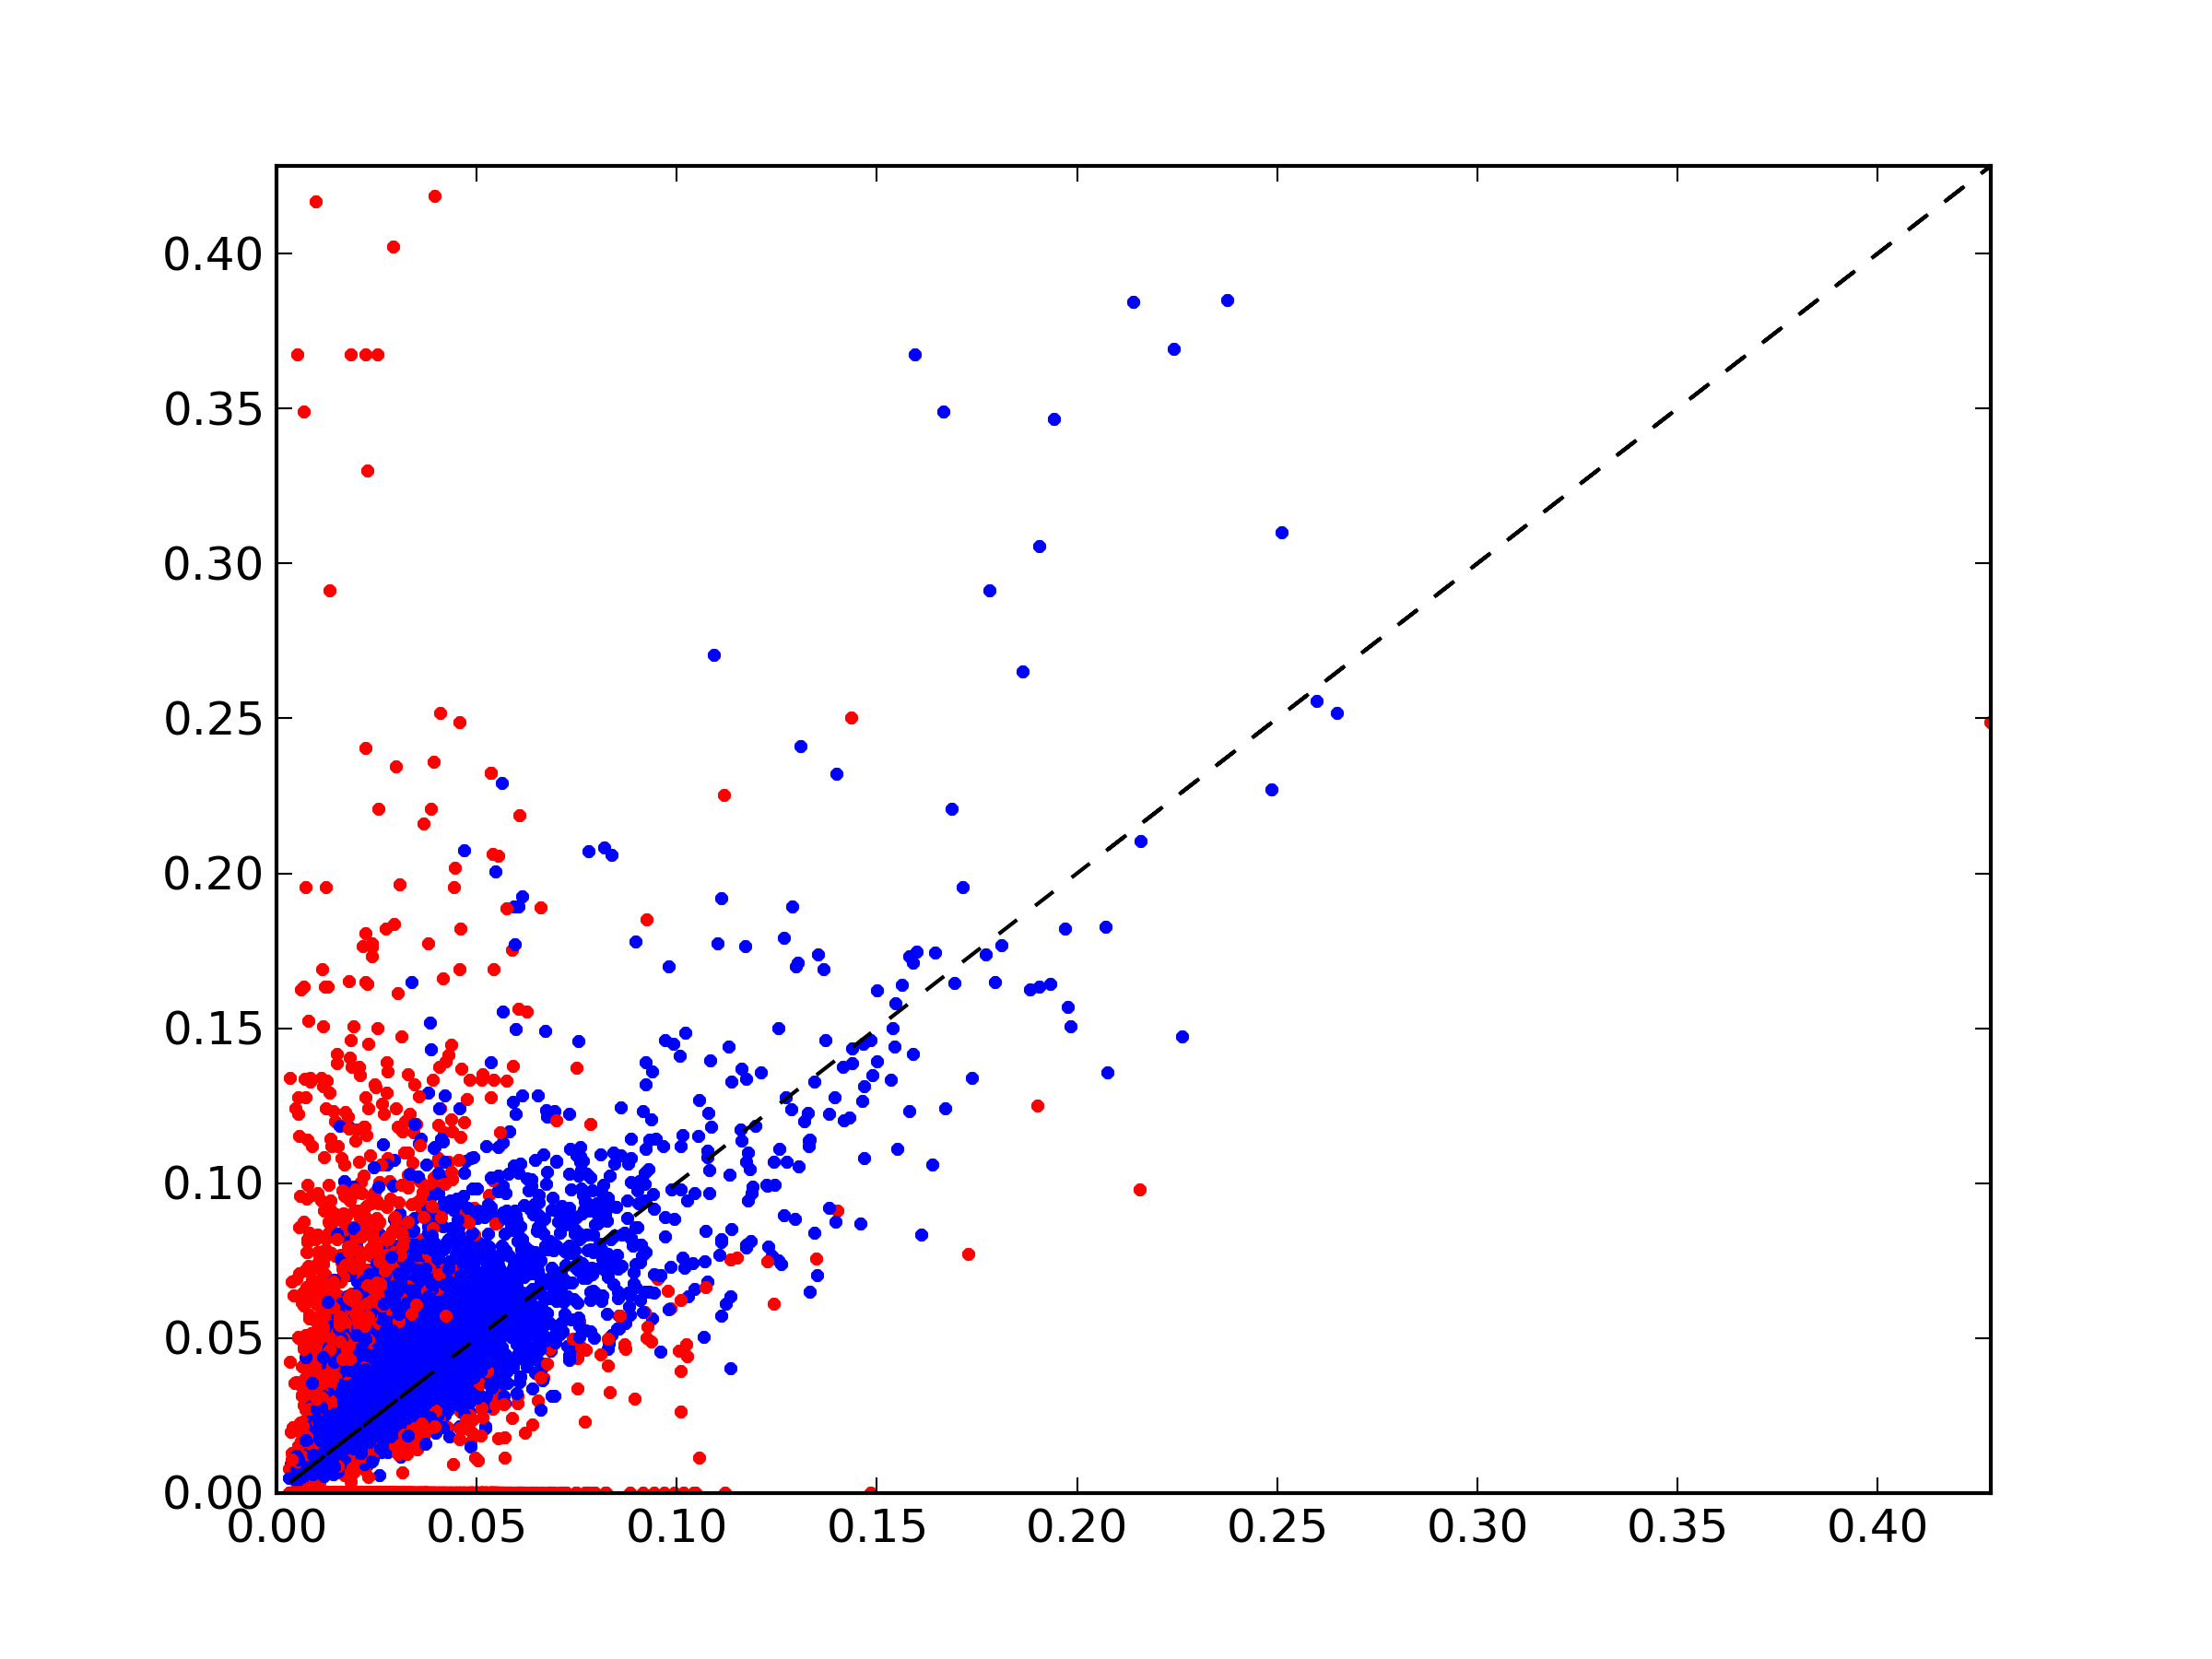
\includegraphics[scale=0.43]{/home/christian/Documentos/git/Montecarlo-NFW/data/results/results_2014-02-11-23:43:20/rs}
\par\end{centering}

\caption{}


\end{figure}



\subsection{What kind of implications (Low resolution simulations, other fitting
algorithms)}


\section{Conclusions}
\end{document}
